\documentclass[11pt,notes=hide,aspectratio=169,mathserif]{beamer}

% PACKAGES
\usepackage{graphics}
\usepackage{graphicx}  % \resizebox
\usepackage{url}
%\usepackage{natbib}
\usepackage{bibentry}
\usepackage{verbatim}
\usepackage{booktabs}
\usepackage{etoolbox}
\usepackage{datetime}
\usepackage{bm}
\usepackage{subcaption}
\usepackage{amsfonts}
\usepackage{amsmath}
\usepackage{amsthm}

% CUSTOM DEFINITIONS
\def\newblock{} % Get beamer to cooperate with BibTeX
\linespread{1.2}

% IDENTIFYING INFORMATION
\title[class]{ECON 340: Economics of the Family \\ TA Session 4}
\author[Vaidehi's class]{Vaidehi Parameswaran (Northwestern Economics)}
\date{\monthname[\the\month] \the\year}

% THEME OPTIONS
\usetheme{metropolis}
\definecolor{mycolor}{RGB}{48,7,144}
\setbeamercolor{frametitle}{bg=mycolor, fg=white}
\setbeamercolor{title separator}{fg=mycolor}
\setbeamercolor{progress bar}{fg=mycolor}
\beamertemplatenavigationsymbolsempty
\setbeamertemplate{footline}[frame number]{}
\setbeamertemplate{itemize item}{\small\raisebox{1pt}{\textcolor{mycolor}{$\blacktriangleright$}}}
\setbeamertemplate{itemize subitem}{\footnotesize\raisebox{1pt}{\textcolor{mycolor}{$\triangleright$}}}
\setbeamertemplate{itemize subsubitem}{\tiny\raisebox{1pt}{\textcolor{mycolor}{$\triangleright$}}}

% Clickable links
\usepackage{hyperref}
\hypersetup{
  colorlinks=true,
  linkcolor=mycolor,
  urlcolor=mycolor,
  citecolor=mycolor
}

% BACKUP SLIDE NUMBERING
\usepackage{appendixnumberbeamer}

% Show a bulleted mini-contents slide at each section
% Bulleted ToC using your triangle icons + color
\setbeamertemplate{section in toc}{%
  \leavevmode\llap{\textcolor{mycolor}{$\blacktriangleright$}\hspace{0.6ex}}%
  \inserttocsection\par}
\setbeamertemplate{subsection in toc}{%
  \leavevmode\llap{\textcolor{mycolor}{$\triangleright$}\hspace{1.1ex}}%
  \inserttocsubsection\par}

\AtBeginSection[]{
  \begin{frame}{Today}
    \tableofcontents[currentsection]
  \end{frame}
}

\begin{document}

%---------------------------------------------------------------------
\begin{frame}[plain]
\titlepage
\end{frame}
%---------------------------------------------------------------------


\section{All the Single Ladies — Folke \& Rickne (AEJ Applied, 2020)}

%---------------------------------------------------------------------
\begin{frame}{Today's Paper}
\small
\textbf{Olle Folke \& Johanna Rickne (2020).} \emph{All the Single Ladies: Job Promotions and the Durability of Marriage}, \textit{AEJ: Applied Economics}, 12(1): 260–87.\\[0.6em]
\begin{itemize}
  \item \textbf{Question:} Do promotions to top jobs change marriage stability? 
  \item \textbf{The punchline:} Promotions \textbf{double the baseline divorce probability for women}, but not for men. 
  \item \textbf{Settings:} Politicians (mayors \& parliamentarians) and \textbf{CEOs}. 
  \item \textbf{Mechanisms preview:} Divorce increases after women’s promotions are concentrated in \textbf{gender-traditional couples}; \textbf{gender-equal couples} are largely unaffected. 
\end{itemize}
{\footnotesize Source: \href{https://www.aeaweb.org/articles?id=10.1257/app.20180435}{aeaweb.org/articles?id=10.1257/app.20180435}}
\end{frame}
%---------------------------------------------------------------------

%---------------------------------------------------------------------
\begin{frame}{Motivation \& Contribution}
\small
\begin{itemize}
  \item Women are severely underrepresented in top positions of organizational hierarchies
  \item In 2017, men accounted for 94 percent of CEOs in Forbes 500 firms and more than 77 percent of the world’s parliamentarians
  \item Inequality translates into gender gaps in income, status, voice, and democratic representation 
  \item It also feeds negative stereotypes about women’s leadership abilities and depresses the career ambitions of young women
\end{itemize}
\end{frame}
%---------------------------------------------------------------------

%---------------------------------------------------------------------
\begin{frame}{Motivation \& Contribution}
\small
\begin{itemize}
  \item Promotions change income, status, hours, travel, and networks—\textbf{all} can shift intra-household preferences/constraints.
  \item Hard to establish causality: promotions are endogenous. 
  \item \textbf{Contribution:} A clean design comparing “\textbf{promoted}” vs “\textbf{almost-promoted}” candidates in \textbf{close elections}, plus evidence from \textbf{CEO} promotions.
  \item Adds to the literature on gender norms, labor market shocks, and family stability.
\end{itemize}
\end{frame}
%---------------------------------------------------------------------

%---------------------------------------------------------------------
\begin{frame}{Why should promotions matter for marriage?}
\small
\begin{itemize}
  \item Bertrand, Kamenica, and Pan 2015: couples in which wife earns more than the husband are more unhappy 
  \item Fisman et al. 2006: uses speed dating experiments to show that men shy away women that they perceive to be smarter or more ambitious than themselves
  \item Bursztyn, Fujiwara, and Pallais 2017: Field experiment on MBA students; single women drastically understated their ambition levels compared to women already
  in relationships when they're told that their reported ambitions will be shared with their classmates (potential suitors)
\end{itemize}
\end{frame}
%---------------------------------------------------------------------

\subsection{Setting, Data, \& Measurement}

%---------------------------------------------------------------------
\begin{frame}{Data \& Outcomes}
\small
\begin{itemize}
  \item \textbf{Setting: Sweden}. Administrative registers cover employment, income, marital status, children, and parental leave.
  \item \textbf{Samples:} (i) Political candidates for mayor/parliament (promotion $\Rightarrow$ winning a seat/office); (ii) \textbf{CEO} promotions.
  \item Why political candidates? Because they can identify who won and who lost
  \item \textbf{Key outcome:} Remaining married / divorce hazard in years relative to promotion.
  \item \textbf{Pre-promotion traits:} relative earnings, parental leave shares, spouse education/age, marriage duration. 
\end{itemize}
\end{frame}
%---------------------------------------------------------------------

%---------------------------------------------------------------------
\begin{frame}{Data \& Outcomes}
\small
\begin{figure}
\centering
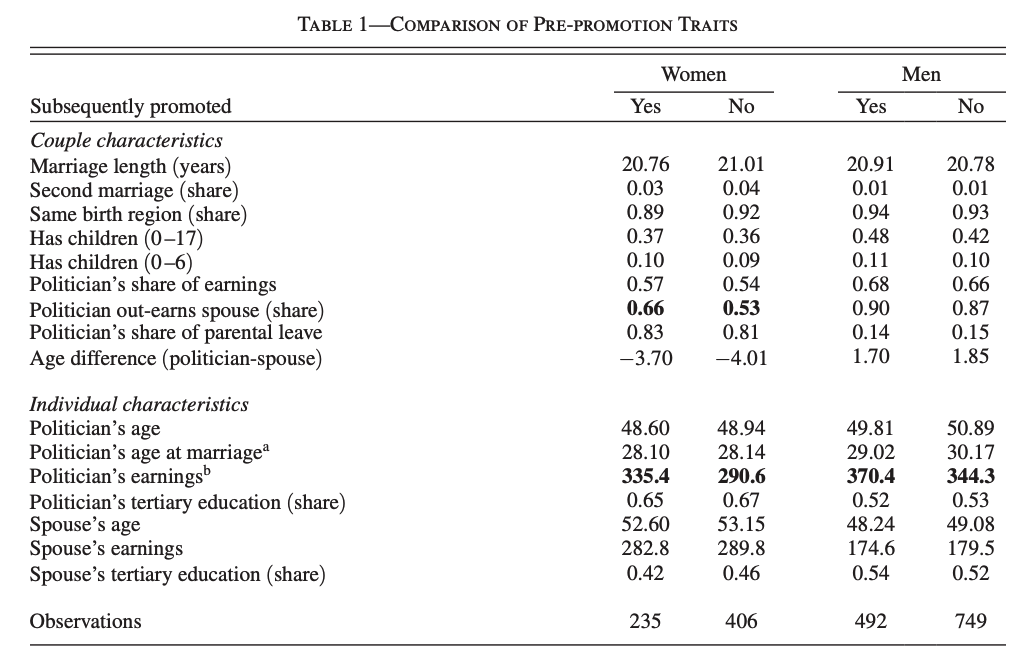
\includegraphics[width=0.8\linewidth]{inputs/table1.png}
\end{figure}
\end{frame}
%---------------------------------------------------------------------



%---------------------------------------------------------------------
\begin{frame}{Identification I: Event-Study DiD}
\small
\[
Y_{iet} = \beta_t P_{ie} T_t + T_t + \delta{ie} + S_{ie} T_t + \tau_e T_t + \varepsilon_{iet},
\]
\begin{itemize}
  \item Dynamic DiD around the promotion year (\(t=0\)); \(\beta_\tau\) trace pre-trends and post effects.
  \item \textbf{Outcome:} remaining married (or divorce hazard) in year \(t\).
  \item Fixed effects for elections ($\tau_E$) 
  \item $\beta$: capture the gap in remaining married between promoted and non-promoted people, relative to the size of that gap in t = 0
\end{itemize}
\end{frame}
%---------------------------------------------------------------------

%---------------------------------------------------------------------
\begin{frame}{Descriptives}
\small
\begin{figure}
\centering
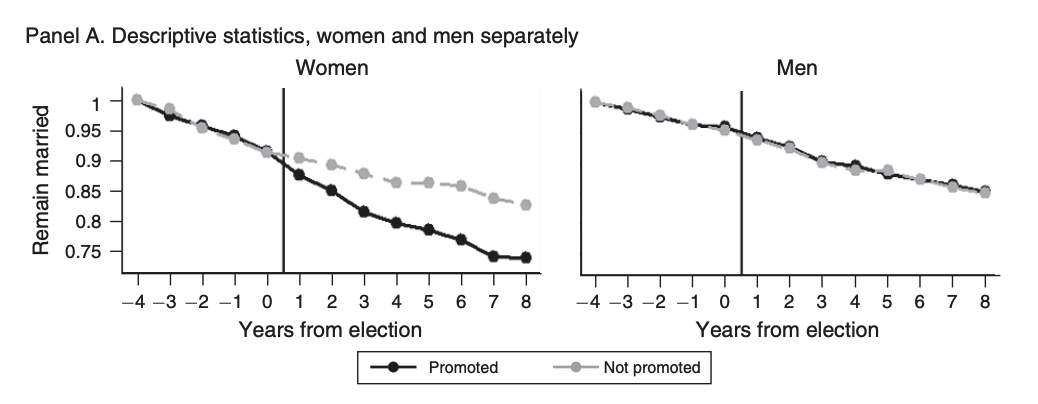
\includegraphics[width=0.8\linewidth]{inputs/fig1.png}
\end{figure}
\end{frame}
%---------------------------------------------------------------------


%---------------------------------------------------------------------
\begin{frame}{Diff-in-diff - the $\beta$s}
\small
\begin{figure}
\centering
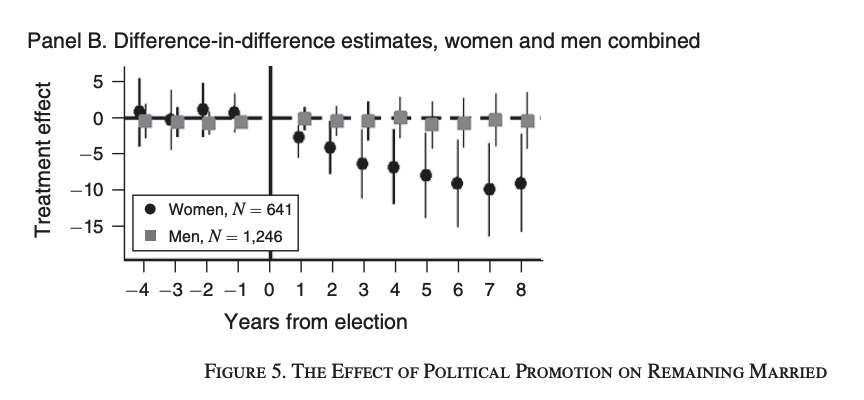
\includegraphics[width=0.8\linewidth]{inputs/fig2.png}
\end{figure}
\end{frame}
%---------------------------------------------------------------------


\subsection{Results}

%---------------------------------------------------------------------
\begin{frame}{Main Result: Women vs. Men}
\small
\begin{itemize}
  \item \textbf{Women:} sharp and sustained \textbf{decline} in probability of being married after promotion. Event-study effects reach roughly \textbf{–7 to –10 pp} by 6–8 years post. 
  \item \textbf{Men:} \textbf{no robust effect} on remaining married in comparable designs. 
  \item \textbf{Interpretation:} Women’s promotions are associated with a \textbf{doubling of baseline divorce risk}; men’s are not. 
\end{itemize}
\end{frame}
%---------------------------------------------------------------------

%---------------------------------------------------------------------
\begin{frame}{Identification II: Close Elections as Quasi-Random Promotions}
\small
\begin{itemize}
  \item There still exists selection problem here - women—but not men—decide to pursue a promotion when their marriage is
  on the rocks
  \item In proportional-representation elections, \textbf{seat majorities} turn on small vote shifts.
  \item Compare \textbf{winners vs runners-up} in “close” contests $\Rightarrow$ promotions are as-good-as-random near the threshold.
\end{itemize}
\end{frame}
%---------------------------------------------------------------------

%---------------------------------------------------------------------
\begin{frame}{Diff-in-diff - the $\beta$s}
\small
\begin{figure}
\centering
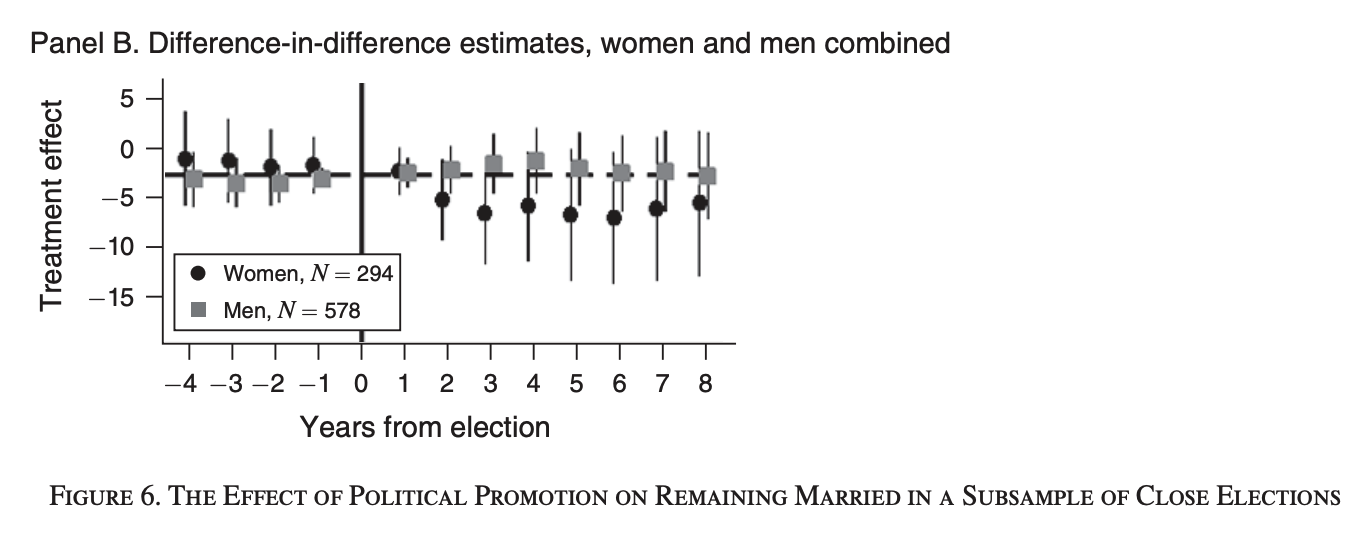
\includegraphics[width=0.8\linewidth]{inputs/fig3.png}
\end{figure}
Qualitatively the same result, less precisely estimated
\end{frame}
%---------------------------------------------------------------------

%---------------------------------------------------------------------
\begin{frame}{Sorting?}
\small
Women with less stable marriages might compete more fiercely to
get elected and perhaps simultaneously strive harder for a promotion in their
job outside  of politics
\begin{figure}
\centering
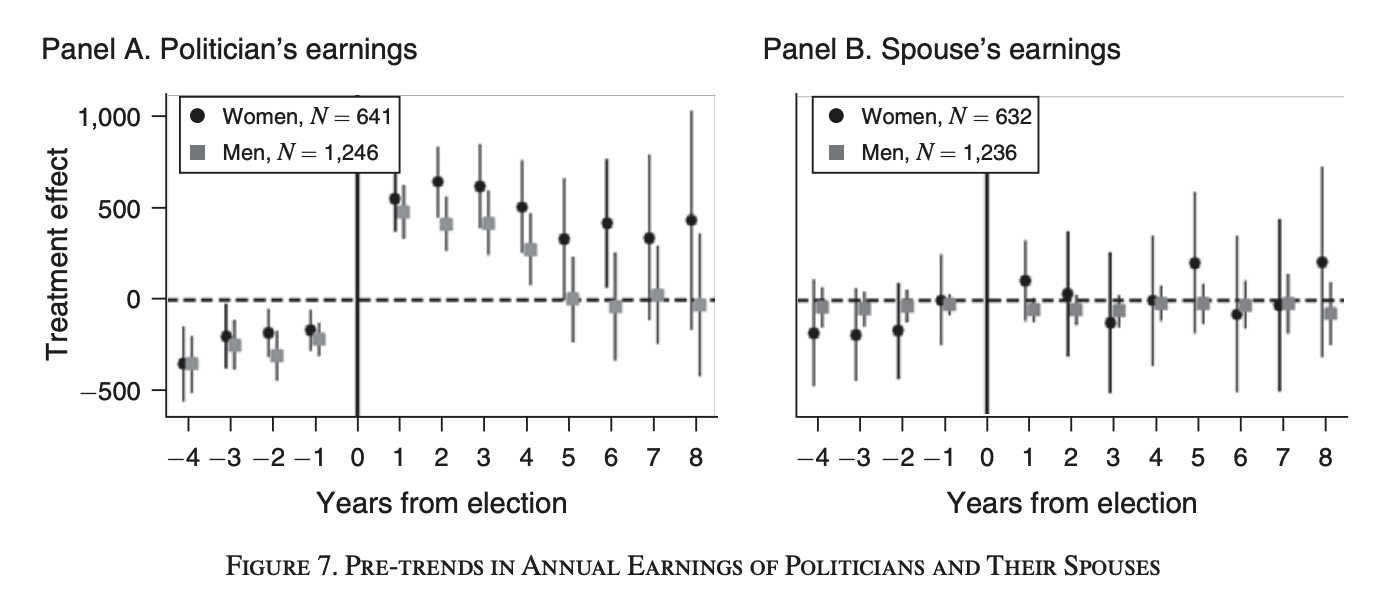
\includegraphics[width=0.8\linewidth]{inputs/fig6.png}
\end{figure}
Not quite
\end{frame}
%---------------------------------------------------------------------


%---------------------------------------------------------------------
\begin{frame}{External Validation: CEOs}
\small
\begin{itemize}
  \item Being a CEO is very prestigious in any firm, typically the pinnacle of a career
  \item Helps generalize beyond political careers (different work environments, selection)
  \item Problem: only observe \textbf{successful} promotions, not “almost-promoted” CEOs
\end{itemize}
\end{frame}
%---------------------------------------------------------------------

%---------------------------------------------------------------------
\begin{frame}{CEO Results}
\small
\begin{figure}
  \centering
  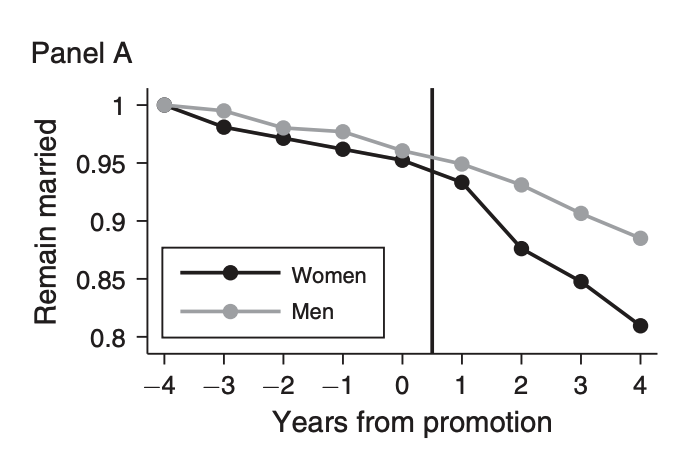
\includegraphics[width=0.6\linewidth]{inputs/fig4.png}
  \end{figure}
\begin{itemize}
  \item Does not permit causal inference
  \item However, very similar to results on politicians
\end{itemize}
\end{frame}
%---------------------------------------------------------------------

%---------------------------------------------------------------------
\begin{frame}{CEO Results}
\small
\begin{figure}
  \centering
  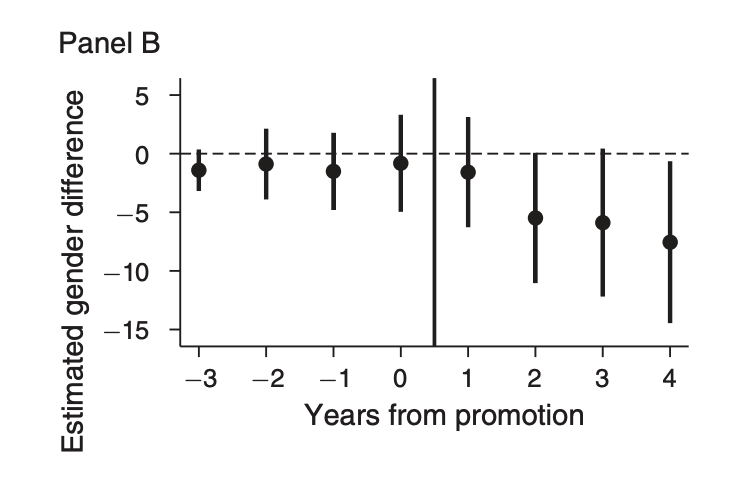
\includegraphics[width=0.5\linewidth]{inputs/fig5.png}
  \end{figure}
\begin{itemize}
  \item Female CEOs who were married at the time of their promotion are more than twice
  as likely to have gotten divorced three years after their promotion
  \item Gender difference is statistically significant at the 5 percent level
  \item Prior to the promotion, the sample shows
  no clear gender difference in rates of divorce
\end{itemize}
\end{frame}
%---------------------------------------------------------------------

%---------------------------------------------------------------------
\begin{frame}{Temptation Effect?}
\small
\begin{itemize}
  \item A promotion can change a person’s work environment and introduce them to
  new  potential partners.
  \item Look at pre-promotion exposure to (opposite-sex) coworkers 
  \item Get ``high'' or ``low'' expected temptation based 
  \item Sample split 
\end{itemize}
\end{frame}
%---------------------------------------------------------------------

%---------------------------------------------------------------------
\begin{frame}{Temptation Effect? A more direct test}
\small
\begin{figure}
  \centering
  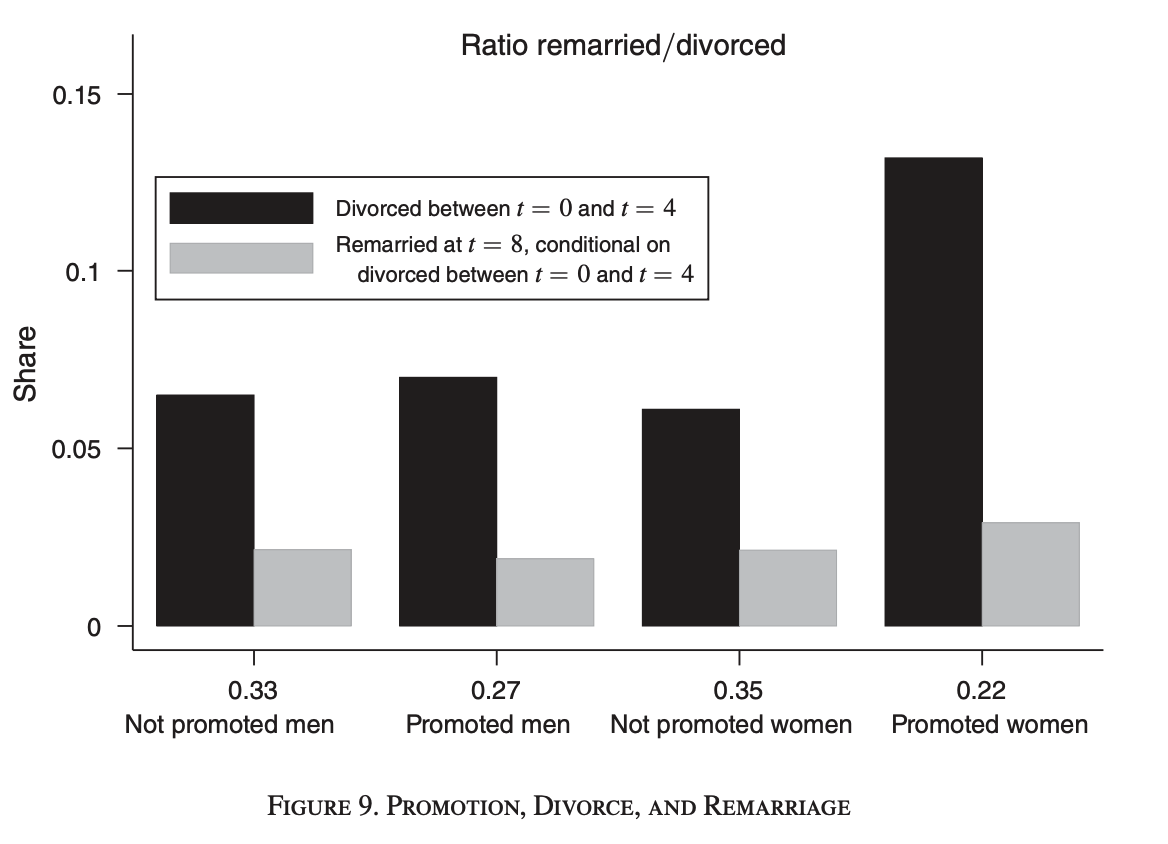
\includegraphics[width=0.8\linewidth]{inputs/fig7.png}
  \end{figure}
\end{frame}
%---------------------------------------------------------------------

%---------------------------------------------------------------------
\begin{frame}{Heterogeneity by Gender Norms}
\small
\begin{itemize}
  \item Marriages may be destabilized if job promotions
  move the division of paid or unpaid labor away from the spouses’ expectations
  of those divisions
  \item Measure couple “\textbf{gender-traditional}” vs “\textbf{gender-equal}” using pre-promotion indicators: 
  \begin{itemize}
    \item Spousal age gap: 3 bins
    \item Division of parental leave: traditional if she took up more than 90\% of leave
  \end{itemize}
  \item \textbf{Result:} Divorce increases are \textbf{concentrated in gender-traditional couples}; \textbf{gender-equal couples} show \textbf{little to no increase}. 
\end{itemize}
\end{frame}
%---------------------------------------------------------------------

%---------------------------------------------------------------------
\begin{frame}{Age Gap}
\small
\begin{figure}
  \centering
  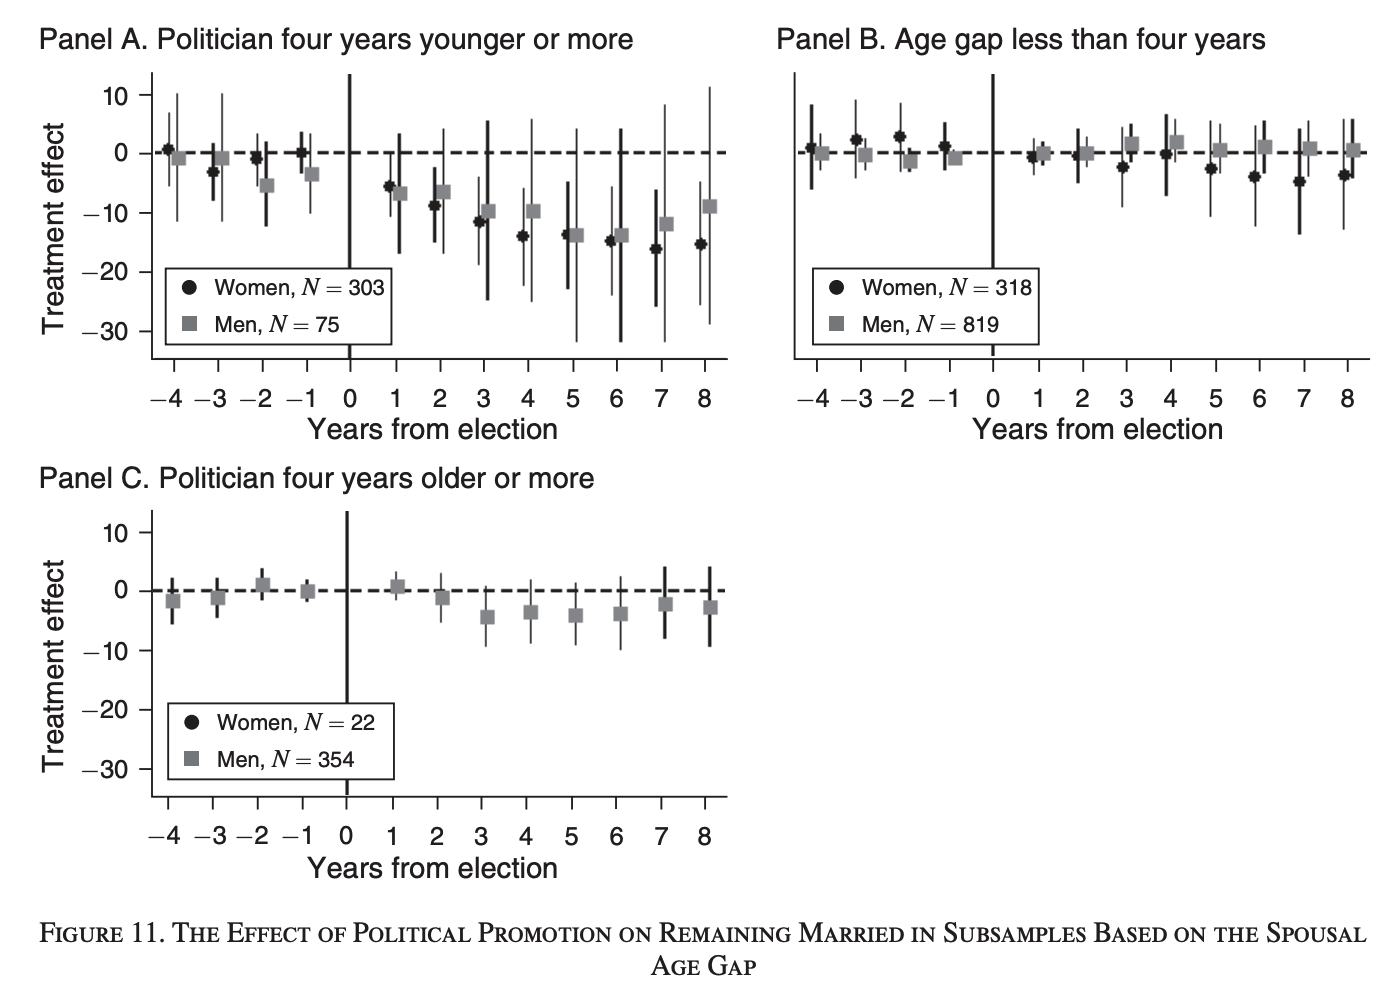
\includegraphics[width=0.8\linewidth]{inputs/fig8.png}
  \end{figure}
\end{frame}
%---------------------------------------------------------------------

%---------------------------------------------------------------------
\begin{frame}{Parental Leave}
\small
\begin{figure}
  \centering
  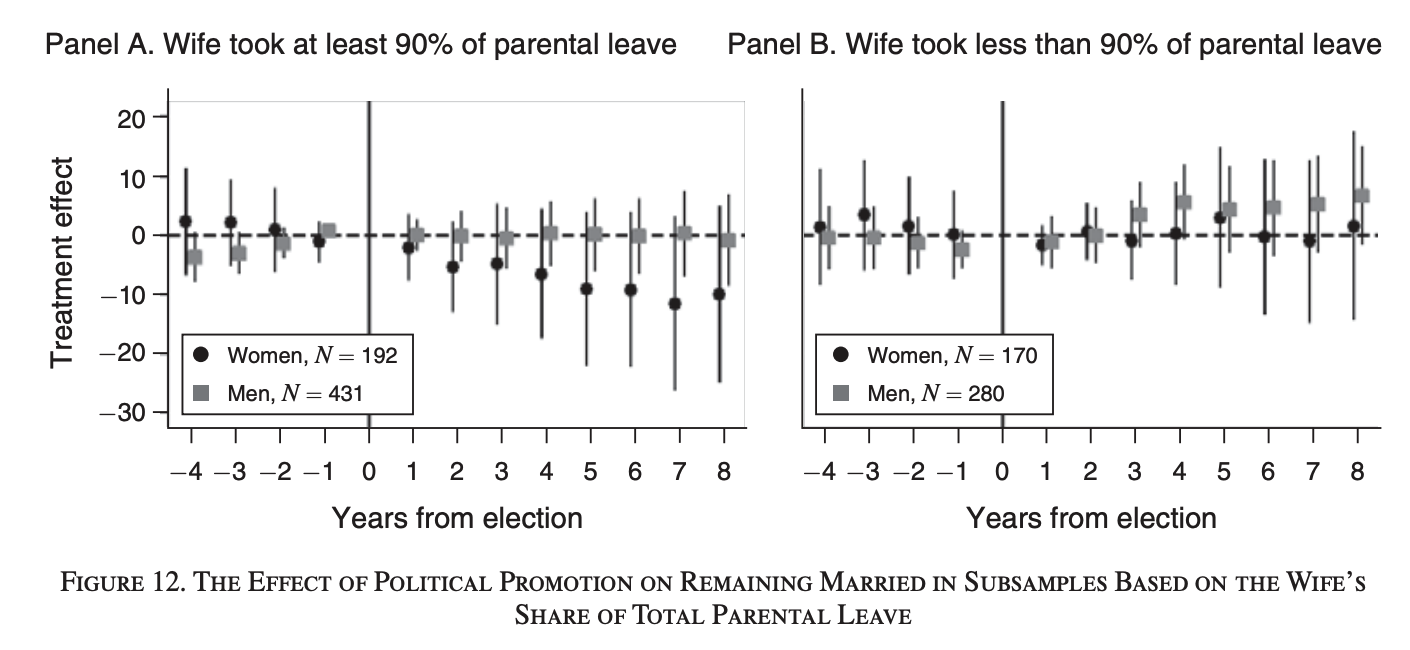
\includegraphics[width=0.8\linewidth]{inputs/fig9.png}
  \end{figure}
\end{frame}
%---------------------------------------------------------------------

%---------------------------------------------------------------------
\begin{frame}{Economic Independence?}
\small
\begin{itemize}
  \item Potential support for this by showing greater sensitivity to women’s than to men’s economic outcomes
  \item Divide the sample based on change in earnings after promotion
  \item Does not seem to be the case - similar effects for high and low earners
  \item This lack of evidence is unsurprising - the women were already high earners before the promotion
\end{itemize}
\end{frame}
%---------------------------------------------------------------------

%---------------------------------------------------------------------
\begin{frame}{Discussion of Mechanisms}
\small
\begin{itemize}
  \item Mechanisms point to the importance of a mismatch
  between expectations  about spousal behavior—in the early phases of the
  relationship—and  actual labor market outcomes as an explanation of women’s
  divorces after promotion.
  \item Couples face adjustment costs when the spouse whose
  career was initially subordinate is promoted
  \item The baseline finding of women’s increased divorce rate after promotion could therefore stem
  from the fact that women more often find themselves in relationships that initially
  focus on the career of the other person, while men do not
\end{itemize}
\end{frame}
%---------------------------------------------------------------------

%---------------------------------------------------------------------
\begin{frame}{Conclusion}
\small
\begin{itemize}
  \item The main result is that promotions destabilize women’s
  marriages but not men’s
  \item  Giving up on the relationship may
  very well be the woman’s choice and may be a positive outcome for her
  \item But highlight a large gender inequality in access to the first-best option for
  most: a functioning relationship and a successful career
  \item The candidate pool for top jobs would be skewed by a condition for women,
  but not for men, to put their relationship at risk
  \item Prioritization
  of the husband’s career remains common around the world, even in progressive
  countries like Sweden
  \item Future research could explore the conditions that allow
  women at the top of the ability distribution to expand their choice set of partners to
  “marry down,” and for men to do the opposite
  \item A less permissive context
  could prohibit  professional women from getting married in the first place
\end{itemize}
\end{frame}
%---------------------------------------------------------------------




% =====================================================
\section{Divorce Law and Marriage-Specific Capital — Stevenson (JLE 2007)}

%---------------------------------------------------------------------
\begin{frame}{Today's Paper}
\small
\textbf{Betsey Stevenson (2007).} \emph{The Impact of Divorce Laws on Marriage-Specific Capital}, \textit{Journal of Labor Economics}, 25(1): 75–94.\\[0.6em]
\begin{itemize}
  \item \textbf{Question:} Do \emph{unilateral} divorce laws change couples’ incentives to invest in \textbf{marriage-specific capital} early in marriage?
  \item \textbf{Design:} Use cross-state legal changes in the \textbf{1970s} as quasi-experimental variation to compare newly married couples before/after adoption of \textbf{unilateral divorce}.
\end{itemize}
\end{frame}
%---------------------------------------------------------------------

%---------------------------------------------------------------------
\begin{frame}{Motivation}
\small
\begin{itemize}
  \item In the 1970s and 1980s, many states adopted unilateral divorce laws
  \item This legal change
  was part of a broader movement in which states began to recognize “irreconcilable differences” as a legitimate reason for divorce
  \item Marriage and divorce laws set the parameters for intertemporal bargaining
  between partners
  \item Couples make decisions - whether or not to have children, how
  many children to have, whether to buy a house, whether one spouse
  should invest in more education, and how to divide home vs market
  work
  \item These affect both the value of their marriage in the future and their
  outside options - central to marriage
\end{itemize}
\end{frame}
%---------------------------------------------------------------------

%---------------------------------------------------------------------
\begin{frame}{Divorce Laws and Marriage-Specific Capital}
\small
\begin{itemize}
  \item If divorce reform raises divorce rates, each spouse is less likely to reap the benefits of marriage-specific capital,
  reducing the incentive to invest jointly
  \item Shifts bargaining power within the household, then
  decisions about marital investments may change, particularly if couples
  differ in their preferences
  \item  The incentive to invest jointly may depend upon the
  ability of the couple to commit to a specific distribution of future rents,
  which is likely shaped by divorce law
  \item Couples may use investment
  in marriage-specific capital strategically—overinvesting today so as to constrain their future selves to prefer to remain married than to divorce
\end{itemize}
\end{frame}
%---------------------------------------------------------------------

%---------------------------------------------------------------------
\begin{frame}{Institutional Background}
\small
\begin{itemize}
  \item \textbf{Unilateral divorce} (``no-fault''): either spouse can dissolve a marriage without proof of wrongdoing.
  \item Staggered adoption across U.S. states during \textbf{late 1960s–1980s} creates variation.
  \item \textbf{Property division regimes} (community property, common law, equitable distribution) shape who shares returns to MSC if divorce occurs.
\end{itemize}
\end{frame}
%---------------------------------------------------------------------

%---------------------------------------------------------------------
\begin{frame}{Empirical Strategy (High-Level)}
\small
\begin{itemize}
  \item Compare \textbf{new marriages} formed in states \emph{before vs. after} unilateral divorce adoption to states that have not yet adopted.
  \item Effect on early-life outcomes: spouse-in-school, fertility in first years, LFP/specialization, home ownership.
  \item \textbf{Difference-in-differences} logic with state and time fixed effects; controls for demographics; robustness to alternative codings of legal changes and to property-law interactions.
\end{itemize}
\end{frame}
%---------------------------------------------------------------------

%---------------------------------------------------------------------
\begin{frame}{Outcomes and Measures}
\small
\begin{itemize}
  \item \textbf{Spouse’s education support:} indicator that one spouse is enrolled while the other works (``putting spouse through school'').
  \item \textbf{Children:} probability of having a child \textbf{within first two years} of marriage; parity in early years.
  \item \textbf{Household specialization:} wife’s labor-force participation; both spouses working full-time vs. one specializing at home.
  \item \textbf{Home ownership:} indicator of owning a home in early marriage; interaction with property-division laws.
\end{itemize}
\end{frame}
%---------------------------------------------------------------------

%---------------------------------------------------------------------
\begin{frame}{Main Results (1): MSC Falls After Unilateral Divorce}
\small
\begin{itemize}
  \item Adoption of \textbf{unilateral divorce} is associated with \textbf{lower} investment in most MSC margins for newlyweds:
  \begin{itemize}
    \item \textbf{Less} ``spouse in school'' support.
    \item \textbf{Lower} likelihood of having a \textbf{birth in first two years} of marriage.
    \item \textbf{Less} household specialization (e.g., \textbf{higher} wife LFP; \textbf{more} both spouses full-time).
  \end{itemize}
  \item Interpreted as a response to a reduced expected surplus from partner-specific investments when \emph{exit becomes easier}.
\end{itemize}
\end{frame}
%---------------------------------------------------------------------

%---------------------------------------------------------------------
\begin{frame}{Main Results (1): MSC Falls After Unilateral Divorce}
\small
\begin{figure}
  \centering
  
\includegraphics[width=0.95\linewidth]{inputs/fig10.png}
  \end{figure}
\end{frame}
%---------------------------------------------------------------------


%---------------------------------------------------------------------
\begin{frame}{Main Results (2): Home Ownership Depends on Property Law}
\small
\begin{itemize}
  \item Unlike other MSC margins, \textbf{home ownership} does \emph{not} uniformly decline.
  \item \textbf{Interaction:} Effect on home ownership depends on \textbf{property-division laws}.
  \item Intuition: If the legal regime \textbf{shares} asset value at divorce, the hold-up risk for a titled asset can be mitigated, preserving (or even encouraging) home investment.
\end{itemize}
\end{frame}
%---------------------------------------------------------------------

%---------------------------------------------------------------------
\begin{frame}{Main Results (2): Home Ownership Depends on Property Law}
\small
\begin{figure}
  \centering
  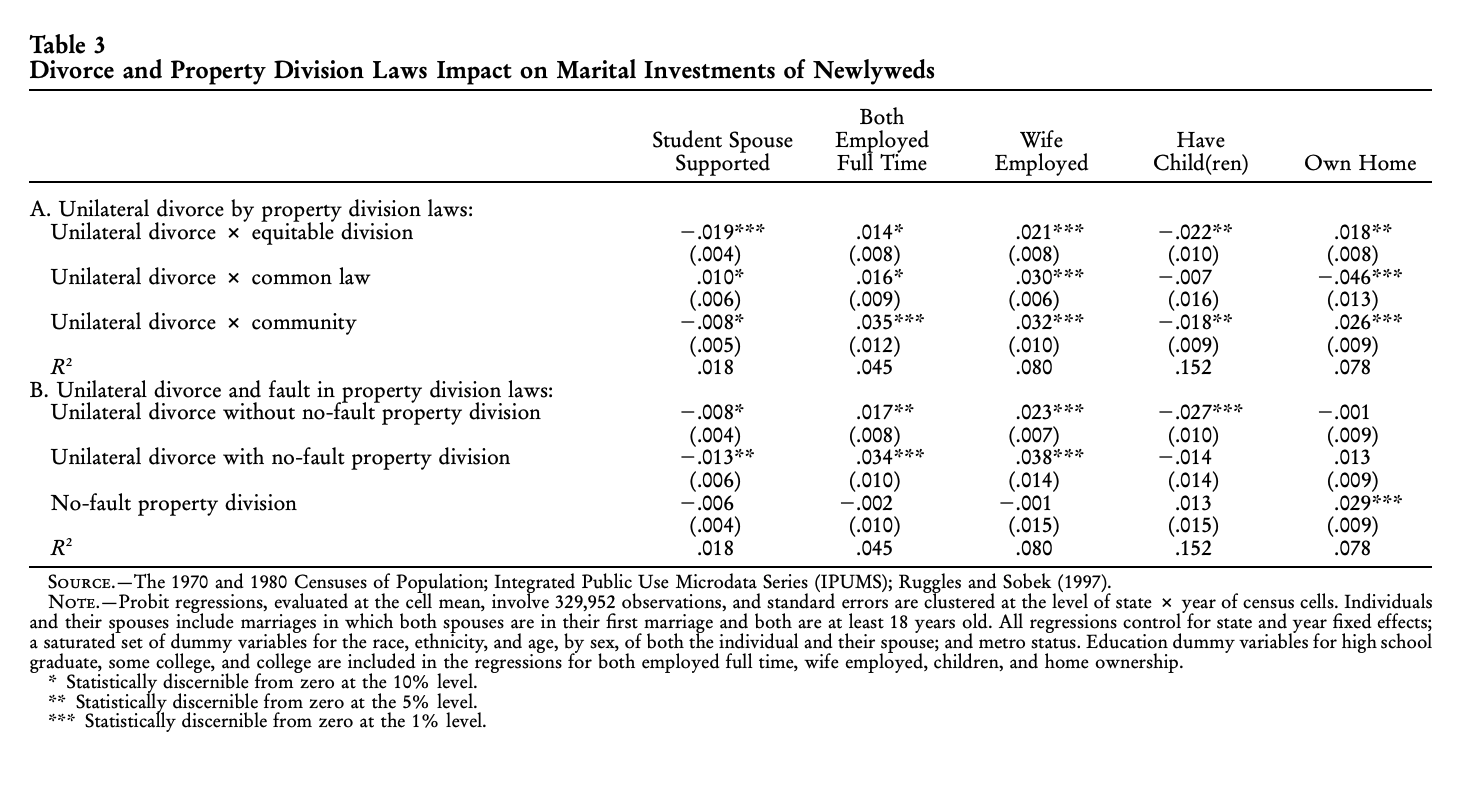
\includegraphics[width=0.95\linewidth]{inputs/fig11.png}
  \end{figure}
\end{frame}
%---------------------------------------------------------------------


% %---------------------------------------------------------------------
% \begin{frame}{Interpreting Magnitudes}
% \small
% \begin{itemize}
%   \item The paper reports economically meaningful reductions in early-life MSC margins after unilateral adoption (exact coefficients vary by specification).
%   \item The \textbf{direction} is consistent across spouse-schooling, fertility timing, and specialization.
%   \item For \textbf{home ownership}, the sign/magnitude hinge on property division—an instructive case where \emph{exit law} and \emph{asset division} interact.
% \end{itemize}
% \end{frame}
% %---------------------------------------------------------------------

%---------------------------------------------------------------------
\begin{frame}{Identification Concerns}
\small
\begin{itemize}
  \item \textbf{Policy endogeneity:} states might adopt unilateral laws amid broader social change.
  \item \textbf{Response:} state/time FE; controls; focusing on \textbf{newlyweds}; robustness to excluding early/late adopters; exploring alternative law codings.
  \item \textbf{Composition effects:} If unilateral divorce changes \emph{who marries}, estimates reflect both selection and behavioral response
\end{itemize}
\end{frame}
%---------------------------------------------------------------------

%---------------------------------------------------------------------
\begin{frame}{Mechanisms \& Economic Intuition}
\small
\begin{itemize}
  \item \textbf{Threat-point shift}: Unilateral divorce raises each spouse’s option value of exit $\Rightarrow$ lowers expected returns to partner-specific investments.
  \item \textbf{Household specialization} becomes riskier (less insurable) when continued marriage is less certain.
  \item \textbf{Asset division rules} can partially \emph{insure} titled investments (e.g., homes), dampening the hold-up.
\end{itemize}
\end{frame}
%---------------------------------------------------------------------

%---------------------------------------------------------------------
\begin{frame}{Policy Takeaways}
\small
\begin{itemize}
  \item Family-law reforms change \textbf{ex-ante} incentives—not just \textbf{ex-post} dissolution rates.
  \item If policymakers value MSC (e.g., early fertility, schooling investments, specialization for childrearing), then \textbf{exit rules} and \textbf{property division} should be considered jointly.
  \item Design implication: \textbf{Complementary} policies (e.g., equitable asset division, portable benefits, or child-related insurance) can protect MSC when exit is easier.
\end{itemize}
\end{frame}
%---------------------------------------------------------------------

%---------------------------------------------------------------------
\begin{frame}{Connecting to the Course Theme}
\small
\begin{itemize}
  \item \textbf{Bargaining in the shadow of the law:} Legal rules set outside options and shape intra-household allocations.
  \item Here: \textbf{divorce law} shifts \emph{ex-ante investment} incentives in marriage.
\end{itemize}
\end{frame}
%---------------------------------------------------------------------

% %---------------------------------------------------------------------
% \begin{frame}{Discussion Prompts}
% \small
% \begin{itemize}
%   \item Which MSC margins are most sensitive to \textbf{exit costs} vs. \textbf{property division}?
%   \item How would you \textbf{separate selection} into marriage from \textbf{behavioral} responses among newlyweds?
%   \item If we ran this design in today’s institutional environment, which margins might move the most (e.g., dual careers, childcare markets)?
% \end{itemize}
% \end{frame}
% %---------------------------------------------------------------------



%---------------------------------------------------------------------
\begin{frame}
\begin{center}{\LARGE See you next time!}\end{center}
\end{frame}
%---------------------------------------------------------------------


\end{document}
